


\modulecomment{

\section{\whatIsTitle?}\label{warmup}

\videoscriptlink{what_is_linear_algebra_overview.mp4}{Video Overview}{video_what_is_overview}

\begin{quote}
Three bears go into a cave, two come out.
Would you go in?

\flushright{Brian Butterworth} 
\vspace{-.2cm}
\begin{center}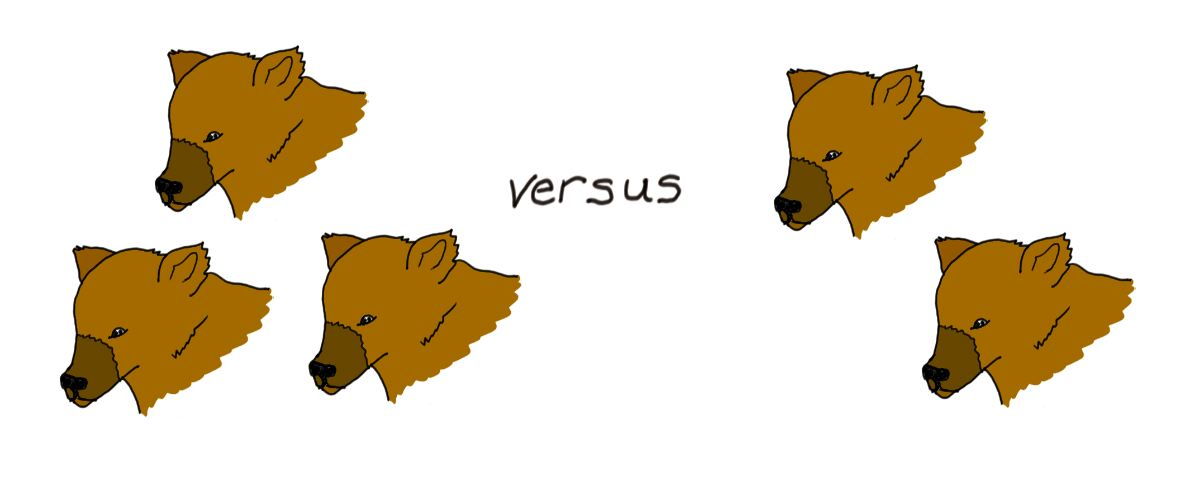
\includegraphics[scale=.21]{bears.jpg}\end{center}
\end{quote}

\noindent
Numbers are highly useful tools for surviving in the modern world, so much so that we often introduce abstract {\it pronumerals} 
to represent them:

\begin{quote}
$n$ bears go into a cave, $n-1$ come out.
Would you go in?
\end{quote}

A single number alone is not sufficient to model more complicated real world situations. For example, suppose I asked everybody in this
room to rate the likeability of everybody else on a scale from 1 to 10. In a room full of $n$ people (or bears {\it sic}) there would be $n^2$ 
ratings to keep track of (how much Jill likes Jill, how much does Jill like Andrew, how much does Andrew like Jill, how much does Andrew like Andrew, {\it etcetera}). We could arrange these in a square array
\begin{equation*}
    \begin{pmatrix}
      9             &4  &\cdots\\
      10             &6 &\\
    \vdots & & \ddots      
    \end{pmatrix}
 \end{equation*}
Would it make sense to replace such an array by an abstract symbol $M$? In the case of numbers, the pronumeral $n$ was more
than a placeholder for a particular piece of information; there exists a myriad of mathematical operations (addition, subtraction, multiplication,...) that can be  performed with the symbol $n$ that could provide useful information about the real world system at hand.
The array $M$ is often called a {\it matrix} and is an example of a more general abstract structure called a {\it linear transformation}
on which many mathematical operations can also be defined.
(To understand why having an abstract theory of linear transformations might be incredibly useful and even lucrative, try replacing ``likeability ratings'' with the number of times internet websites link to one another!)
In this course, we'll learn about three main topics: Linear Systems, Vector Spaces, and Linear Transformations.  Along the way we'll learn about matrices and how to manipulate them.  

For now, we'll illustrate some of  the basic ideas of the course in the case of two by two matrices.  Everything will carefully defined later, we just want
to start with some simple examples to get an idea of the things we'll be working with.

%\modulecommentend
}


\moduletitle{Gaussian Elimination}


\moduleobjectives{
Objectives: 
\begin{enumerate}
\item
Given a multivariable problem, write it as a linear system of equations (when this is possible).
\item
Express a linear system of equations as a  single equation involving matrices and vectors.
\item
Write matrix equations in the shorthand augmented matrix notation.
\item
Understand that different augmented matrices can correspond to the same solution(s).
\item
Know which row operations leave the solutions of an augmented matrix unchanged.
\item 
Understand the reduced row echelon form of an augmented matrix and how to extract solutions from it.
\item
Gaussian elimination: systematically apply row operations to an augmented matrix to obtain reduced row echelon form.

\end{enumerate}
\newpage
}

\modulesection{Linear Systems}

\modulesubsection{A Simple Linear System}


\katvideolink{Lecture_01_WhatIsLinearAlgebra.mp4}{Reading Guide}

\begin{example}
Suppose I have a bunch of apples and oranges.  Let $x$ be the number of apples  and $y$ be the number of oranges.  As everyone knows, apples and oranges don't mix, so if I want to keep track of the number of apples and oranges I have, I should put them in a list.  We'll call this list a \emph{vector,}\index{Vector!in ${\mathbb R}^2$} and write it like this: $(x,y)$.  The order here matters!  I should remember to always write the number of apples first and then the number of oranges--otherwise if I see the vector $(1,2)$, I won't know whether I have two apples or two oranges.
\end{example}

\begin{center}
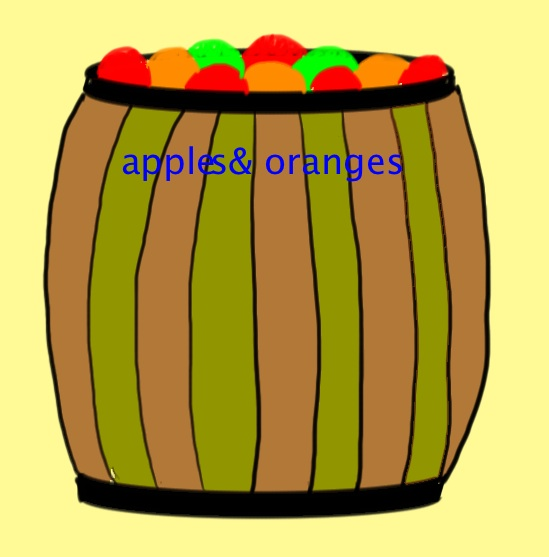
\includegraphics[scale=.3]{\whatIsPath/barrel1.jpg}
\end{center}

The vector~$(x,y)$ in the example is just a list of two numbers, so if we want to, we can represent it as a point in the plane with the corresponding coordinates, like so:

\vspace{2mm}
\begin{center}
\begin{tikzpicture}[domain=0:4]
    \draw[->] (-0.2,0) -- (4.2,0) node[right] {$\mbox{Apples}$};
    \draw[->] (0,-1.2) -- (0,4.2) node[above] {$\mbox{Oranges}$};
    \draw[->] (0,0) -- (2,3) node[anchor=south east] {$(x,y)$};
\end{tikzpicture}
\end{center}
In the plane, we can imagine each point as some combination of apples and oranges (or parts thereof, for the points that don't have integer coordinates).  So each point corresponds to some vector.  The collection of all such vectors---all the points in our apple-orange plane---is an example of a \emph{vector space}.

\begin{example}  There are 27 pieces of fruit in a barrel, and twice as many oranges as apples.  How many apples and oranges are in the barrel?

How to solve this conundrum?  We can re-write the question mathematically as follows:

\begin{eqnarray*}
	x+y & = & 27 \\
	\phantom{x+}y & = & 2x
\end{eqnarray*}
\end{example}

This is an example of a \emph{Linear System}\index{Linear System!concept of}.  It's a collection of equations in which variables are multiplied by constants and summed, and no variables are multiplied together:  There are no powers of $x$ or $y$ greater than one, no fractional or negative powers of $x$ or $y$, and no places where $x$ and $y$ are multiplied together.
%\begin{center}\href{\webworkurl ReadingHomework1/1/}{Reading homework: problem 1.1}\end{center}
\reading{1}{1}

Notice that we can solve the system by manipulating the equations involved.  First, notice that the second equation is the same as $-2x+y=0$.  Then if you subtract the second equation from the first, you get on the left side $x+y - (-2x+y) = 3x$, and on the left side you get $27-0=27$.  Then $3x=27$, so we learn that $x=9$.  Using the second equation, we then see that $y=18$.  Then there are 9 apples and 18 oranges.

Let's do it again, by working with the list of equations as an object in itself.  First we rewrite the equations tidily:

\begin{eqnarray*}
	x+y & = & 27 \\
	2x-y & = & 0
\end{eqnarray*}

We can express this set of equations with a matrix as follows:

\begin{equation*}
    \begin{pmatrix}
      1             &1  \\
      2             &-1
    \end{pmatrix}
  \colvec{x \\ y}
  =
  \colvec{27 \\ 0}
\end{equation*}

The square list of numbers is an example of a \emph{matrix}.  We can multiply the matrix by the vector to get back the linear system using the following rule for multiplying matrices by vectors:

\begin{equation}\label{2x2multiplication}
    \begin{pmatrix}
      a             &b  \\
      c             &d
    \end{pmatrix}
  \colvec{x \\ y}
  =
  \colvec{ax+by \\ cx+dy}
\end{equation}
%\begin{center} \href{\webworkurl ReadingHomework1/2/}{Reading homework: problem 1.2}\end{center}
\reading{1}{2}
\noindent
The matrix is an example of a \emph{Linear Transformation}\index{Linear Transformation!concept of}, because it takes one vector and turns it into another in a ``linear'' way.
Of course, we can have much larger matrices if our system has more variables:

\videoscriptlink{what_is_linear_algebra_3_3_matrix.mp4}{A $3 \times 3$ matrix example}{scripts_what_is_linear_algebra_3_3_matrix}


Our next task is to solve linear systems. We'll learn a general method called Gaussian Elimination.





\References{

Hefferon, Chapter One, Section 1
\\
Beezer, Chapter SLE, Sections WILA and SSLE
\\
Wikipedia, \href{http://en.wikipedia.org/wiki/System_of_linear_equations}{Systems of Linear Equations}
}


\inputProblems{\whatIsPath/problems}

\newpage
